\documentclass[conference]{IEEEtran}
\IEEEoverridecommandlockouts

% Fonts are the IEEE template's own: the class selects Times (ptm) and we add no font
% package. T1 encoding is required because XeTeX otherwise defaults to Unicode (TU), where
% ptm has no bold shape -- \textbf then silently degrades to regular weight, and the body
% text falls back to Latin Modern rather than Times.
\usepackage[T1]{fontenc}
\usepackage{cite}
\usepackage{amsmath,amssymb,amsfonts}
\usepackage{graphicx}
\usepackage{booktabs}
\usepackage{textcomp}
\usepackage{url}

\renewcommand{\figurename}{Fig.}   % match the in-text "Fig.~\ref" style
\graphicspath{{figs/}}
% AUTO-GENERATED by evidence/code/export_numbers.py -- DO NOT EDIT BY HAND.
% Regenerate with: make numbers

\newcommand{\statAbBaseBio}{24.5\%}
\newcommand{\statAbBaseCyber}{34.8\%}
\newcommand{\statAbCritCIBio}{[-2.3, +0.1]}
\newcommand{\statAbCritCICyber}{[-6.3, -3.1]}
\newcommand{\statAbCritDeltaBio}{-1.1}
\newcommand{\statAbCritDeltaCyber}{-4.7}
\newcommand{\statAbShufLetterBio}{26.2\%}
\newcommand{\statAbShufLetterCyber}{31.2\%}
\newcommand{\statAbShufPosBio}{24.8\%}
\newcommand{\statAbShufPosCyber}{30.5\%}
\newcommand{\statAbStateCIBio}{[-0.9, +0.8]}
\newcommand{\statAbStateCICyber}{[-3.3, -0.8]}
\newcommand{\statAbStateDeltaBio}{-0.1}
\newcommand{\statAbStateDeltaCyber}{-2.0}
\newcommand{\statAbSymAccCIBio}{[-1.7, +0.2]}
\newcommand{\statAbSymAccCICyber}{[-2.4, +0.5]}
\newcommand{\statAbSymAccDeltaBio}{-0.8}
\newcommand{\statAbSymAccDeltaCyber}{-1.0}
\newcommand{\statAbSymBio}{25.1\%}
\newcommand{\statAbSymCyber}{36.1\%}
\newcommand{\statAccBio}{85.2\%}
\newcommand{\statAccBioRobust}{80.1\%}
\newcommand{\statAccCyber}{63.4\%}
\newcommand{\statAccProtocol}{53.7\%}
\newcommand{\statAccSupp}{36.6\%}
\newcommand{\statAtkBestRotBio}{89.5\%}
\newcommand{\statAtkBestRotCyber}{79.9\%}
\newcommand{\statAtkDropIdentBio}{1.3}
\newcommand{\statAtkDropIdentCyber}{3.2}
\newcommand{\statAtkDropRotBio}{5.4}
\newcommand{\statAtkDropRotCyber}{14.0}
\newcommand{\statAtkNDatasets}{7}
\newcommand{\statAtkNItemsBio}{1{,}273}
\newcommand{\statAtkNItemsCyber}{1{,}987}
\newcommand{\statAtkNMixedWidth}{2}
\newcommand{\statAtkNSignificant}{7}
\newcommand{\statAtkOrderDropBio}{4.2}
\newcommand{\statAtkOrderDropCIBio}{[3.0, 5.3]}
\newcommand{\statAtkOrderDropCICyber}{[9.4, 12.4]}
\newcommand{\statAtkOrderDropCyber}{10.9}
\newcommand{\statAtkOrderMax}{26.9}
\newcommand{\statAtkOrderMin}{7.4}
\newcommand{\statAtkOrderSteerBio}{7.5}
\newcommand{\statAtkOrderSteerCyber}{24.2}
\newcommand{\statAtkSingleBio}{85.4\%}
\newcommand{\statAtkSingleCyber}{63.3\%}
\newcommand{\statAtkSteerIdentBio}{2.0\%}
\newcommand{\statAtkSteerIdentCyber}{6.5\%}
\newcommand{\statAtkSteerRotBio}{9.5\%}
\newcommand{\statAtkSteerRotBioRobust}{10.4\%}
\newcommand{\statAtkSteerRotChem}{15.4\%}
\newcommand{\statAtkSteerRotCyber}{30.6\%}
\newcommand{\statAtkWorstIdentBio}{84.1\%}
\newcommand{\statAtkWorstIdentCyber}{60.1\%}
\newcommand{\statAtkWorstLabel}{LB-DbQA}
\newcommand{\statAtkWorstRotBio}{80.0\%}
\newcommand{\statAtkWorstRotCyber}{49.2\%}
\newcommand{\statAtkWorstSteer}{32.7\%}
\newcommand{\statAurocBio}{0.855}
\newcommand{\statAurocCyber}{0.774}
\newcommand{\statAurocMax}{0.86}
\newcommand{\statAurocMin}{0.62}
\newcommand{\statAurocPooled}{0.820}
\newcommand{\statAurocPooledHi}{0.830}
\newcommand{\statAurocPooledLo}{0.810}
\newcommand{\statAurocSpread}{0.006}
\newcommand{\statBreakevenBio}{0.672}
\newcommand{\statBreakevenCyber}{0.401}
\newcommand{\statBreakevenLitQA}{0.287}
\newcommand{\statBrierPmax}{0.161}
\newcommand{\statCascadeAdvantageBio}{+0.3}
\newcommand{\statCascadeAdvantageForty}{+2.2}
\newcommand{\statCascadeCostSaving}{45\%}
\newcommand{\statCascadeCyberAtForty}{67.0\%}
\newcommand{\statCascadeCyberAtTwenty}{65.9\%}
\newcommand{\statCascadeCyberCallsForty}{2.2}
\newcommand{\statCascadeCyberRandForty}{64.8\%}
\newcommand{\statCascadeFracOfGain}{97\%}
\newcommand{\statCascadeRandBeatBio}{6.8\%}
\newcommand{\statCascadeRandBeatCyber}{0.0\%}
\newcommand{\statChanceSupp}{21.3\%}
\newcommand{\statCircMixedList}{LB-SeqQA, LB-LitQA2}
\newcommand{\statCircNDatasets}{7}
\newcommand{\statCollectionDates}{\mbox{2026-09-19} to \mbox{2026-09-20}}
\newcommand{\statConfAltEntropy}{20.7\%}
\newcommand{\statConfAltMargin}{31.0\%}
\newcommand{\statConfAltPmax}{28.0\%}
\newcommand{\statConfExample}{0.33}
\newcommand{\statConfMatch}{97.9\%}
\newcommand{\statConfTol}{0.015}
\newcommand{\statConsistBio}{89.4\%}
\newcommand{\statConsistCyber}{62.6\%}
\newcommand{\statDistinctProbs}{101}
\newcommand{\statEceAdaptivePooled}{0.033}
\newcommand{\statEceAdaptiveSupp}{0.185}
\newcommand{\statEceConf}{0.091}
\newcommand{\statEceLitQA}{0.168}
\newcommand{\statEceMax}{0.193}
\newcommand{\statEceMin}{0.033}
\newcommand{\statEcePmax}{0.034}
\newcommand{\statEcePmaxHi}{0.045}
\newcommand{\statEcePmaxLo}{0.027}
\newcommand{\statEceRatio}{2.7}
\newcommand{\statEceSpreadMax}{0.193}
\newcommand{\statEceSpreadMin}{0.033}
\newcommand{\statEceSupp}{0.193}
\newcommand{\statEceWorstWmdp}{0.057}
\newcommand{\statEnsAccCyber}{67.1\%}
\newcommand{\statEnsGainBio}{+0.5}
\newcommand{\statEnsGainBioHi}{+1.4}
\newcommand{\statEnsGainBioLo}{-0.2}
\newcommand{\statEnsGainCyber}{+3.8}
\newcommand{\statEnsGainCyberHi}{+5.3}
\newcommand{\statEnsGainCyberLo}{+2.4}
\newcommand{\statErrGivenHiBio}{3.9\%}
\newcommand{\statErrGivenHiCyber}{7.5\%}
\newcommand{\statErrGivenHiLitQA}{38.1\%}
\newcommand{\statErrGivenHiLitQACI}{[21,\,59]}
\newcommand{\statErrGivenHiSupp}{25.0\%}
\newcommand{\statErrRatioBio}{4.64}
\newcommand{\statErrRatioCyber}{2.93}
\newcommand{\statErrStableCyber}{21.3\%}
\newcommand{\statErrUnstableCyber}{62.5\%}
\newcommand{\statExcessBio}{6.7}
\newcommand{\statExcessCyber}{25.8}
\newcommand{\statFisherBioCyberP}{0.00469}
\newcommand{\statFisherBioCyberQ}{0.0141}
\newcommand{\statFlipCWBio}{6.3\%}
\newcommand{\statFlipCWCyber}{22.2\%}
\newcommand{\statFlipIdenticalBio}{1.34\%}
\newcommand{\statFlipIdenticalCyber}{4.03\%}
\newcommand{\statFlipIdenticalCyberCI}{[3.2,\,5.0]}
\newcommand{\statFlipWCBio}{28.0\%}
\newcommand{\statFlipWCCyber}{45.2\%}
\newcommand{\statHiGivenErrBio}{17.5\%}
\newcommand{\statHiGivenErrCyber}{5.6\%}
\newcommand{\statHiGivenErrLitQA}{6.7\%}
\newcommand{\statInconsistCyber}{37.4\%}
\newcommand{\statInputTokens}{21.6}
\newcommand{\statLabMax}{61.8\%}
\newcommand{\statLabMaxName}{seq}
\newcommand{\statLabMin}{36.6\%}
\newcommand{\statLabMinName}{supp}
\newcommand{\statLiftBio}{0.802}
\newcommand{\statLiftCyber}{0.512}
\newcommand{\statLlmCheapRatio}{1.3}
\newcommand{\statLlmCheapUsd}{1.14}
\newcommand{\statLlmMidRatio}{144}
\newcommand{\statLlmMidUsd}{131}
\newcommand{\statLlmTopRatio}{720}
\newcommand{\statLlmTopUsd}{654}
\newcommand{\statMajAccCyber}{65.2\%}
\newcommand{\statModelVersion}{jev-1.13.0}
\newcommand{\statNBootCI}{2{,}000}
\newcommand{\statNCallsAblation}{13{,}040}
\newcommand{\statNCallsAll}{67{,}245}
\newcommand{\statNCallsCircular}{23{,}145}
\newcommand{\statNCallsSingle}{6{,}020}
\newcommand{\statNCallsTotal}{29{,}165}
\newcommand{\statNCircItemsBio}{1{,}273}
\newcommand{\statNCircItemsCyber}{1{,}987}
\newcommand{\statNCompared}{1{,}987}
\newcommand{\statNDatasets}{10}
\newcommand{\statNDisagreeCyber}{80}
\newcommand{\statNErrors}{1}
\newcommand{\statNHiBio}{848}
\newcommand{\statNHiCyber}{550}
\newcommand{\statNHiLitQA}{21}
\newcommand{\statNHiSupp}{8}
\newcommand{\statNItems}{6{,}020}
\newcommand{\statNItemsRaw}{6{,}021}
\newcommand{\statNSigPosDatasets}{3}
\newcommand{\statNTestedPosDatasets}{8}
\newcommand{\statNTied}{71}
\newcommand{\statNoisePredBio}{4.0\%}
\newcommand{\statNoisePredCyber}{11.6\%}
\newcommand{\statNoiseShareBio}{37\%}
\newcommand{\statNoiseShareCyber}{31\%}
\newcommand{\statNullRatioBio}{10.03}
\newcommand{\statNullRatioBioCI}{[8.31, 12.61]}
\newcommand{\statNullRatioCyber}{5.43}
\newcommand{\statNullRatioCyberCI}{[4.68, 6.35]}
\newcommand{\statNullRatioCyberHi}{6.35}
\newcommand{\statNullRatioCyberLo}{4.68}
\newcommand{\statPermAllBio}{17.4\%}
\newcommand{\statPermAllCyber}{46.8\%}
\newcommand{\statPermCyclicBio}{11.0\%}
\newcommand{\statPermCyclicCyber}{37.2\%}
\newcommand{\statPermMatchedCIBio}{[-2.4, +2.0]}
\newcommand{\statPermMatchedCICyber}{[-4.8, +0.8]}
\newcommand{\statPermMatchedDiffBio}{-0.2}
\newcommand{\statPermMatchedDiffCyber}{-2.0}
\newcommand{\statPermNItemsBio}{500}
\newcommand{\statPermNItemsCyber}{500}
\newcommand{\statPermNOrderingsBio}{24}
\newcommand{\statPermNOrderingsCyber}{24}
\newcommand{\statPermNonCyclicBio}{10.8\%}
\newcommand{\statPermNonCyclicCyber}{35.2\%}
\newcommand{\statPermSteerAllBio}{15.8\%}
\newcommand{\statPermSteerAllCyber}{39.8\%}
\newcommand{\statPermUndercountBio}{1.6}
\newcommand{\statPermUndercountCyber}{1.3}
\newcommand{\statPermWorstAllBio}{74.8\%}
\newcommand{\statPermWorstAllCyber}{43.8\%}
\newcommand{\statPosChiCyber}{79.7}
\newcommand{\statPosGoldACyber}{26.6\%}
\newcommand{\statPosHighGoldA}{27.8\%}
\newcommand{\statPosHighP}{0.84}
\newcommand{\statPosHighPower}{1.00}
\newcommand{\statPosHighPredA}{27.5\%}
\newcommand{\statPosLowGoldA}{21.8\%}
\newcommand{\statPosLowP}{<10^{-4}}
\newcommand{\statPosLowPredA}{42.5\%}
\newcommand{\statPosNullCrit}{7.2}
\newcommand{\statPosPBio}{0.11}
\newcommand{\statPosPCyber}{<10^{-4}}
\newcommand{\statPosPowerBio}{1.00}
\newcommand{\statPosPredACyber}{34.8\%}
\newcommand{\statRCBioAtSixty}{0.971}
\newcommand{\statRCBioAtSixtyPct}{97.1\%}
\newcommand{\statRCBioBase}{0.852}
\newcommand{\statRCCyberAtSixty}{0.789}
\newcommand{\statRCCyberAtSixtyPct}{78.9\%}
\newcommand{\statRCCyberBase}{0.634}
\newcommand{\statReBetweenBio}{9.8\%}
\newcommand{\statReBetweenCyber}{37.8\%}
\newcommand{\statReCalls}{25{,}040}
\newcommand{\statReFacItems}{500}
\newcommand{\statReFacRepeats}{3}
\newcommand{\statReGainDiffBio}{+0.6}
\newcommand{\statReGainDiffCIBio}{[-0.2, +1.4]}
\newcommand{\statReGainDiffCICyber}{[+2.0, +4.8]}
\newcommand{\statReGainDiffCyber}{+3.4}
\newcommand{\statReGainIdentBio}{-0.1}
\newcommand{\statReGainIdentCyber}{+0.5}
\newcommand{\statReGainRotBio}{+0.5}
\newcommand{\statReGainRotCyber}{+3.8}
\newcommand{\statReGapBio}{8.2}
\newcommand{\statReGapCyber}{28.2}
\newcommand{\statReIdentBio}{2.4\%}
\newcommand{\statReIdentCyber}{9.2\%}
\newcommand{\statReNoiseShareBio}{23\%}
\newcommand{\statReNoiseShareCyber}{25\%}
\newcommand{\statReRatioBio}{3.8}
\newcommand{\statReRatioCyber}{4.8}
\newcommand{\statReRepeats}{4}
\newcommand{\statReRotBio}{10.6\%}
\newcommand{\statReRotCyber}{37.4\%}
\newcommand{\statReWithinBio}{2.5\%}
\newcommand{\statReWithinCyber}{7.8\%}
\newcommand{\statRevFlipMax}{34.2\%}
\newcommand{\statRevFlipMin}{6.8\%}
\newcommand{\statRevMaxAccChange}{9.8}
\newcommand{\statRevNChanged}{none}
\newcommand{\statRevNDatasets}{10}
\newcommand{\statRotSpreadBio}{1.3}
\newcommand{\statRotSpreadCyber}{0.8}
\newcommand{\statSingleAccCyber}{63.3\%}
\newcommand{\statThrBioOnBio}{5.0\%}
\newcommand{\statThrBioOnCyber}{9.0\%}
\newcommand{\statThrBioWorst}{40.0\%}
\newcommand{\statThrBioWorstLabel}{LB-LitQA2}
\newcommand{\statThrBioWorstN}{25}
\newcommand{\statThrBioWorstRatio}{8.0}
\newcommand{\statThrCovBio}{69\%}
\newcommand{\statThrCovCyber}{24\%}
\newcommand{\statThrNAchievable}{5}
\newcommand{\statThrNDatasets}{10}
\newcommand{\statThrNUnachievable}{5}
\newcommand{\statThrTarget}{5\%}
\newcommand{\statThrTauBio}{0.87}
\newcommand{\statThrTauCyber}{0.94}
\newcommand{\statThrUnachievableList}{LB-CloningScenarios, LB-DbQA, LB-LitQA2, LB-ProtocolQA, LB-SuppQA}
\newcommand{\statTieContainingFirst}{46}
\newcommand{\statTieExpectedFirst}{23.0}
\newcommand{\statTieFrac}{1.2\%}
\newcommand{\statTieObservedFirst}{21}
\newcommand{\statTieTotal}{71}
\newcommand{\statTokensPerCall}{741}
\newcommand{\statUsdPerM}{0.042}
\newcommand{\statUsdTotal}{0.91}
\newcommand{\statVerAccNewBio}{85.1\%}
\newcommand{\statVerAccNewCyber}{64.0\%}
\newcommand{\statVerAccOldBio}{85.2\%}
\newcommand{\statVerAccOldCyber}{63.4\%}
\newcommand{\statVerAnyAccChanged}{no}
\newcommand{\statVerDisagreeBio}{4.6\%}
\newcommand{\statVerDisagreeCyber}{13.9\%}
\newcommand{\statVerDisagreeMax}{13.9\%}
\newcommand{\statVerDisagreeMin}{4.6\%}
\newcommand{\statVerPBio}{1}
\newcommand{\statVerPCyber}{0.43}
\newcommand{\statVerPublished}{jev-1.13.0}
\newcommand{\statVerReplication}{jev-1.14.0}
\newcommand{\statVerSteerNewBio}{9.5\%}
\newcommand{\statVerSteerNewCyber}{26.0\%}
\newcommand{\statVerSteerOldBio}{9.5\%}
\newcommand{\statVerSteerOldCyber}{30.6\%}


\newcommand{\jev}{\textsc{Jev}}
\newcommand{\pmax}{p_{\max}}

% The reference list runs to twenty entries on a six-page limit. IEEEtran leaves a blank
% line between entries by default; removing it recovers most of a column and changes
% nothing about the content. Done here rather than by dropping references.
\let\oldthebibliography\thebibliography
\renewcommand{\thebibliography}[1]{%
  \oldthebibliography{#1}%
  \setlength{\itemsep}{0pt}%
  \setlength{\parsep}{0pt}%
  \setlength{\parskip}{0pt}}

% IEEEtran hardcodes an em-dash after the keywords label, so the separator cannot be
% changed by redefining \IEEEkeywordsname alone. This copies the compsoc-conference
% branch of the environment verbatim and substitutes a colon.
\makeatletter
\def\IEEEkeywords{\normalfont\@IEEEtweakunitybaselinestretch{1.15}\bfseries
    \if@twocolumn
      \@IEEEabskeysecsize\vskip 0.5\baselineskip plus 0.25\baselineskip minus 0.25\baselineskip\noindent
      \textit{\IEEEkeywordsname:}\ \relax
    \else
      \bgroup\par\addvspace{0.5\baselineskip}\centering\@IEEEabskeysecsize\textbf{\IEEEkeywordsname}\par\addvspace{0.5\baselineskip}\egroup\quotation\@IEEEabskeysecsize%
    \fi\@IEEEgobbleleadPARNLSP}
\makeatother

\special{pdf:minorversion 4}
\begin{document}

\title{Auditing System-1 Models on Biosecurity-Relevant Benchmarks:\\
Calibration, Selective Prediction, and Permutation Instability\\
in a Non-Generative Model}

\author{%
\IEEEauthorblockN{Kimon Antonios Provatas \qquad
                  Ilias Georgakopoulos-Soares}
\thanks{Corresponding author: Ilias Georgakopoulos-Soares.}
\IEEEauthorblockA{Division of Pharmacology and Toxicology, College of Pharmacy\\
The University of Texas at Austin, Dell Pediatric Research Institute\\
Austin, TX, USA\\
kap4722@my.utexas.edu \qquad ilias@austin.utexas.edu}
}

\maketitle

\begin{abstract}
Non-generative ``System-1'' models return structured probabilistic decisions in a single
forward pass, without autoregressive decoding, at a small fraction of the inference cost of
a generative model. This makes them of interest as inexpensive components in larger
pipelines, but their reliability on biosecurity-relevant tasks has not been systematically
examined. We audit one commercial System-1 model on \statNItems{} multiple-choice items
drawn from the Weapons of Mass Destruction Proxy (WMDP), a paraphrase-robust WMDP-Bio
variant, and six LAB-Bench subtasks, measuring accuracy, calibration, error detection,
selective prediction, and sensitivity to the order in which answer options are presented.
Accuracy is strongly task-dependent. Once the vendor's uncertainty field is correctly
interpreted --- it rescales the top-1 probability and is not a probability of being correct
--- the model is reasonably well calibrated (pooled ECE \statEcePmax{}) and separates
correct from incorrect predictions (pooled AUROC \statAurocPooled{}), but neither pooled
figure is safe to deploy against: a cutoff set on WMDP-Bio to hold errors at
\statThrTarget{} delivers \statThrBioWorst{} errors on \statThrBioWorstLabel{}, and on
\statThrNUnachievable{} of \statThrNDatasets{} tasks no cutoff reaches that target at any
coverage. Treating answer order as something an adversary controls, worst-case WMDP-Cyber
accuracy falls from \statAtkSingleCyber{} to \statAtkWorstRotCyber{} and
\statAtkSteerRotCyber{} of items are correct under some orderings and incorrect under
others; a budget-matched control using byte-identical repeated calls attributes
\statAtkOrderDropCyber{} of that \statAtkDropRotCyber{}~percentage-point drop to order
rather than run-to-run variation, and the effect holds on all
\statAtkNDatasets{} datasets tested, on option counts from 2 to 10, and across a vendor
version update that leaves accuracy unchanged while altering
\statVerDisagreeCyber{} of decisions.
\end{abstract}

\begin{IEEEkeywords}
model evaluation, calibration, selective prediction, robustness, biosecurity, AI safety
\end{IEEEkeywords}

\section{Introduction}

Recent work on efficient inference has produced models that return a typed, probabilistic
decision from a single forward pass rather than by decoding tokens autoregressively. Such
``System-1'' models are offered for settings in which many decisions must be made cheaply.
The evaluation reported here cost \statUsdTotal{}~USD for \statNCallsTotal{} calls, against
roughly \statLlmCheapUsd{}--\statLlmTopUsd{}~USD for the same items with a generative model
at list prices (Section~\ref{sec:setup}). That difference is what makes repeated evaluation
of the same item a practical experimental option rather than a hypothetical one.

Low-cost probabilistic models are potentially relevant to AI safety and biosecurity
pipelines, where auxiliary classifiers are already deployed alongside larger
models~\cite{llamaguard,constclass}. Before such a role could be considered, the basic
empirical properties of these models need to be established: how accurate they are, how
well their reported uncertainty tracks correctness, whether that uncertainty supports
abstention, and how stable their decisions are under changes that do not alter the meaning
of the input. Benchmark accuracy addresses only the first of these.

This paper reports a reliability audit of one commercially available System-1 model,
\jev{}, on two kinds of benchmark. The Weapons of Mass Destruction Proxy
(WMDP)~\cite{wmdp} covers biosecurity, chemical security and cybersecurity, written as a
measurable stand-in for knowledge that could assist misuse and introduced so that
unlearning methods could be scored on \emph{reducing} it; high accuracy on it is therefore
not a capability result. LAB-Bench~\cite{labbench} covers practical biology research skill
and carries the opposite sign. Neither asks the model to judge whether a request is
dangerous, so neither measures screening or hazard-detection performance; they are subject
matter on which reliability, uncertainty and robustness can be studied.

\noindent Our contributions are properties that a benchmark score cannot expose, and a
measurement protocol that exposes them.
\begin{enumerate}
\item \textbf{A protocol for auditing a scored decision API}, which first establishes what
      the vendor's uncertainty field actually measures. Here it is an affine rescaling of
      the top-1 probability, not a probability of being correct; scoring calibration
      against the documented field reports \statEceConf{} expected calibration error where
      the true figure is \statEcePmax{}. The check costs three lines of code and applies to
      any model behind a scored interface.
\item \textbf{Answer order is a decision-steering surface.} Someone who controls only the
      order the options are listed in, and nothing about their content, can move
      \statAtkSteerRotCyber{} of WMDP-Cyber decisions. A budget-matched control using
      byte-identical repeated calls separates this from endpoint non-determinism, which
      prior order-sensitivity work does not do.
\item \textbf{Confidence cutoffs do not transfer across tasks.} A cutoff fitted on one
      dataset misses its error target by up to \statThrBioWorstRatio{}$\times$ on another,
      and on \statThrNUnachievable{} of \statThrNDatasets{} tasks no cutoff meets a
      \statThrTarget{} error target at any coverage --- so a pooled calibration figure is
      the wrong basis for an operating threshold.
\end{enumerate}
\noindent We also report that averaging over answer orderings, applied selectively to
low-confidence items, recovers most of the accuracy lost to instability at a fraction of
the cost of averaging every item.

We do not claim novelty for confidence-based selection of items for further
computation~\cite{calm,bild,frugalgpt,routellm}, nor for the observation that
multiple-choice evaluation is sensitive to option order~\cite{alzahrani,gupta}.

\section{Background and Related Work}

\textbf{Decision cascades and early exit.} Spending extra computation only on inputs a
cheap model finds difficult is established: CALM~\cite{calm} exits a decoder early under a
calibrated criterion, Big Little Decoder~\cite{bild} escalates when a small model's maximum
predicted probability falls below a threshold, and FrugalGPT~\cite{frugalgpt} and
RouteLLM~\cite{routellm} allocate queries across models under a cost budget. Our final
experiment applies the same idea with additional answer permutations rather than a larger
model. For uncertainty we use standard tools: maximum class probability as an
error-detection baseline~\cite{hendrycks}, expected calibration error and reliability
diagrams~\cite{guo}, and risk--coverage analysis~\cite{geifman}.

\textbf{Multiple-choice robustness.} Reordering answer options changes model rankings on leaderboards~\cite{alzahrani} and
degrades accuracy in model-dependent ways~\cite{gupta}; Zheng et al.~\cite{zheng}
attribute the effect to a token-level bias toward particular option labels, and
formatting changes that preserve meaning can also shift accuracy
substantially~\cite{formatspread}. That work concerns generative models scored by likelihood
over option tokens. We test whether a non-generative model emitting a typed distribution in
one pass shows comparable sensitivity.

\textbf{Safety classifiers and biosecurity context.} Deployed language-model systems
commonly place auxiliary classifiers around a primary model to detect disallowed content:
moderation classifiers~\cite{openaimod}, input--output safeguards such as Llama
Guard~\cite{llamaguard} and ShieldGemma~\cite{shieldgemma}, and constitutional classifiers
trained to resist jailbreaks~\cite{constclass}, with biological risk a specific
concern~\cite{biorisk}. That work motivates why inexpensive probabilistic models are of
interest, but we evaluate none of these safeguard tasks: prior work asks whether a system
can block a dangerous request, whereas we ask what reliability properties a cheap System-1
model exhibits on biosecurity-relevant knowledge benchmarks.

\section{Experimental Setup}
\label{sec:setup}

\jev{} is a commercial non-generative model queried through the \texttt{v1} REST endpoint.
A request carries a free-text state and a typed question; the response gives a selected
category, a probability distribution over categories, a scalar \texttt{confidence}, the
resolved model version, and token usage. All calls used the alias \texttt{jev-latest},
which resolved to \texttt{\statModelVersion{}} throughout, and were made from
\statCollectionDates{}. The model is proprietary: no logits, token probabilities, or random
seed are exposed, and returned probabilities are quantised to two decimals
(\statDistinctProbs{} distinct values observed). We did not measure latency and make no
claim about it.

Table~\ref{tab:main} lists the \statNDatasets{} datasets. WMDP-Bio, WMDP-Chem and
WMDP-Cyber are hazardous-knowledge proxies~\cite{wmdp}, WMDP-Bio-Robust is a paraphrased
variant of WMDP-Bio, and six LAB-Bench subtasks cover practical biology
research~\cite{labbench}. Option counts range from 2 to 10, so we report accuracy against
each item's own chance level $1/n$ rather than a single 25\% line. LAB-Bench items combine
the reference answer with its distractors under a fixed shuffle seed; items with fewer than
two distinct options after de-duplication are skipped. Of \statNItemsRaw{} single-pass
calls, \statNErrors{} returned an API error and is excluded, leaving \statNItems{} items.

We report accuracy; expected calibration error (ECE) over ten equal-width bins; the area
under the receiver operating characteristic curve (AUROC) for separating correct from
incorrect predictions using $\pmax$, the largest returned probability; the error rate
conditional on high confidence, $P(\text{error} \mid \pmax \geq 0.9)$; and risk--coverage
curves obtained by withholding the least confident items. Intervals on proportions are
Wilson; those on ECE, AUROC and accuracy differences are percentile bootstrap over items,
\statNBootCI{} resamples with a fixed seed. For the two four-option WMDP suites we
additionally present each item under all four cyclic rotations of its option list
($\statNCircItemsBio{}$ and $\statNCircItemsCyber{}$ items, \statNCallsCircular{} calls),
mapping each returned distribution back to the original option indices so that rotations
are comparable.

The endpoint reports token usage per response. The study consumed
\statInputTokens{}~million input tokens over \statNCallsTotal{} calls at
\statUsdPerM{}~USD per million, with no output charge: \statUsdTotal{}~USD in total,
against \statLlmCheapUsd{}--\statLlmTopUsd{}~USD for the same calls with a generative
model at list prices retrieved 2026-09-20
(\statLlmCheapRatio{}--\statLlmTopRatio{}$\times$). Those are upper bounds, since batch
interfaces list at half rate and cached input at a tenth. We did not measure latency.

\begin{table*}[t]
\centering
\caption{Per-dataset results. ECE and AUROC are on $p_{\max}$, not the vendor \texttt{confidence} field. \emph{Retained} withholds the least confident 40\%. \emph{Flip} is the share of predictions that change when the option list is reversed, a single meaning-preserving change: no dataset's accuracy moves significantly, yet up to a third of decisions do. Intervals are Wilson.}
\label{tab:main}
\footnotesize
\setlength{\tabcolsep}{3.3pt}
\begin{tabular}{@{}llrccccccc@{}}
\toprule
Suite & Dataset & $N$ & opts. & accuracy [95\% CI] & ECE & AUROC & $P(\text{err}\mid p_{\max}\!\geq\!0.9)$ & retained & flip \\
\midrule
WMDP & WMDP-Bio & 1273 & 4 & 0.852 [0.83, 0.87] & 0.036 & 0.855 & 0.039 [0.03, 0.05] & 0.971 & 0.068 \\
 & WMDP-Bio-Robust & 811 & 4 & 0.801 [0.77, 0.83] & 0.044 & 0.823 & 0.063 [0.04, 0.09] & 0.938 & 0.085 \\
 & WMDP-Chem & 408 & 4 & 0.730 [0.69, 0.77] & 0.057 & 0.824 & 0.056 [0.03, 0.10] & 0.898 & 0.127 \\
 & WMDP-Cyber & 1987 & 4 & 0.634 [0.61, 0.66] & 0.033 & 0.774 & 0.075 [0.06, 0.10] & 0.789 & 0.268 \\
\midrule
LAB-Bench & LB-CloningScenarios & 32 & 4--8 & 0.469 [0.31, 0.64] & 0.126 & 0.671 & 0.500 [0.09, 0.91] & 0.579 & 0.281 \\
 & LB-ProtocolQA & 108 & 4--7 & 0.537 [0.44, 0.63] & 0.124 & 0.620 & 0.077 [0.01, 0.33] & 0.600 & 0.241 \\
 & LB-SeqQA & 600 & 2--5 & 0.618 [0.58, 0.66] & 0.093 & 0.861 & 0.000 [0.00, 0.05] & 0.825 & 0.295 \\
 & LB-DbQA & 520 & 4 & 0.398 [0.36, 0.44] & 0.086 & 0.653 & 0.091 [0.03, 0.28] & 0.468 & 0.342 \\
 & LB-LitQA2 & 199 & 2--10 & 0.402 [0.34, 0.47] & 0.168 & 0.656 & 0.381 [0.21, 0.59] & 0.479 & 0.236 \\
 & LB-SuppQA & 82 & 4--8 & 0.366 [0.27, 0.47] & 0.193 & 0.709 & 0.250 [0.07, 0.59] & 0.429 & 0.341 \\
\midrule
\multicolumn{2}{@{}l}{\textbf{pooled}} & 6020 & 2--10 & 0.673 [0.661, 0.685] & 0.034 & 0.820 & -- & -- & -- \\
\bottomrule
\end{tabular}
\end{table*}


\section{Results}

\subsection{Benchmark performance and uncertainty}
\label{sec:uncertainty}

Accuracy varies widely across tasks (Table~\ref{tab:main}). It is highest on WMDP-Bio
(\statAccBio{}), falls on the paraphrased WMDP-Bio-Robust (\statAccBioRobust{}), and is
substantially lower on WMDP-Cyber (\statAccCyber{}). LAB-Bench results are lower and more variable, from \statLabMin{} on SuppQA to
\statLabMax{} on SeqQA; SuppQA is the weakest subtask, though still above its
\statChanceSupp{} chance level. Aggregate accuracy therefore describes the
particular task at least as much as the model.

Interpreting the model's uncertainty requires first establishing what the reported
\texttt{confidence} field measures. Across all \statNItems{} records it matches
$c = (\pmax - 1/n)/(1 - 1/n)$, where $n$ is the number of options, to within
$\pm\statConfTol{}$ for \statConfMatch{} of records. Competing readings fit less well: raw
$\pmax$ matches \statConfAltPmax{}, the top-two margin \statConfAltMargin{}, and
normalised entropy \statConfAltEntropy{}. The field rescales the top-1 probability onto
$[0,1]$, mapping a uniform distribution to 0 and a one-hot one to 1, so on a four-option
item an even split between two candidates ($\pmax = 0.5$) is reported as
\statConfExample{}. It is not a predicted probability of correctness, and calibration
should be assessed against $\pmax$.

On that basis, pooled ECE is \statEcePmax{} (95\% CI $[\statEcePmaxLo{},
\statEcePmaxHi{}]$; Brier \statBrierPmax{}), against \statEceConf{} when the rescaled
field is used (Fig.~\ref{fig:uncertainty}(a)). Pooled AUROC for separating correct from
incorrect predictions is \statAurocPooled{} (95\% CI $[\statAurocPooledLo{},
\statAurocPooledHi{}]$), so $\pmax$ carries information about correctness. Both pooled
figures flatter the model, since pooling lets $\pmax$ discriminate partly on which dataset
an item came from: per-task values span \statAurocMin{}--\statAurocMax{} AUROC and
\statEceMin{}--\statEceMax{} ECE (Table~\ref{tab:main}), and those are the relevant figures
for a system consuming these predictions. Four candidate signals --- $\pmax$, the top-two
margin, negative entropy, and the rescaled field --- differ by at most
\statAurocSpread{} AUROC, so the choice among them is not consequential.

\begin{figure*}[t]
\centering
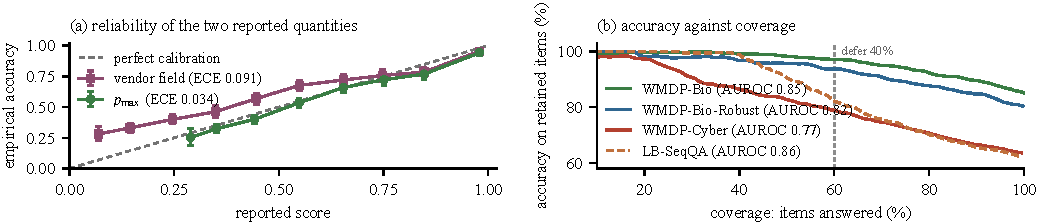
\includegraphics[width=\textwidth]{fig1_uncertainty.pdf}
\caption{Uncertainty and selective prediction. (a) Pooled reliability curves for the two
quantities the API reports: the \texttt{confidence} field (squares) is an affine
rescaling of $\pmax$ (circles), so calibration measured against it differs from
calibration measured against the probability itself. Bins holding fewer than 25 items
are omitted, because $\pmax \geq 1/n$ leaves the lowest bins of the $\pmax$ curve nearly
empty; error bars are Wilson intervals. (b) Accuracy on retained items against coverage,
withholding the least confident first, for the three WMDP suites and the largest LAB-Bench subtask (dashed); the remaining six subtasks are omitted for legibility and appear
in Table~\ref{tab:main}. The dashed vertical marker is the 40\% deferral operating point
quoted in Section~\ref{sec:selective} and in Table~\ref{tab:main}.}
\label{fig:uncertainty}
\end{figure*}

\subsection{Confidence and selective prediction}
\label{sec:selective}

A quantity directly interpretable for a system consuming these predictions is the error
rate given a confident answer. Under $P(\text{error} \mid \pmax \geq 0.9)$ the model is
most reliable on WMDP-Bio (\statErrGivenHiBio{}, $n=\statNHiBio{}$) and less so on
WMDP-Cyber (\statErrGivenHiCyber{}, $n=\statNHiCyber{}$); a Fisher exact test gives $p =
\statFisherBioCyberP{}$, and $q = \statFisherBioCyberQ{}$ after Benjamini--Hochberg
correction across all pairwise comparisons. Confident answers are much less reliable on the
LAB-Bench literature tasks, reaching \statErrGivenHiLitQA{} on LitQA2 ($n=\statNHiLitQA{}$).
Withholding low-confidence items raises accuracy on the remainder
(Fig.~\ref{fig:uncertainty}(b)): deferring the least confident 40\% raises the retained set
from \statAccBio{} to \statRCBioAtSixtyPct{} on WMDP-Bio and from \statAccCyber{} to
\statRCCyberAtSixtyPct{} on WMDP-Cyber, so confidence does identify a subset on which the
model performs substantially better.

That is a prerequisite for deferral, but not enough to set an operating threshold, because
the threshold itself does not transfer. We fit, on each dataset, the lowest $\pmax$ cutoff
holding errors among accepted items at or below \statThrTarget{}, then apply it unchanged
elsewhere. The cutoff fitted on WMDP-Bio is $\statThrTauBio{}$, accepting
\statThrCovBio{} of items at the intended \statThrBioOnBio{} error rate; the same cutoff
yields \statThrBioOnCyber{} on WMDP-Cyber and \statThrBioWorst{} on
\statThrBioWorstLabel{} ($n = \statThrBioWorstN{}$ accepted), a
\statThrBioWorstRatio{}$\times$ miss. More restrictive still, on \statThrNUnachievable{} of
\statThrNDatasets{} datasets --- \statThrUnachievableList{} --- \emph{no} cutoff reaches a
\statThrTarget{} error rate at any coverage. For those tasks the honest operating answer is
that this model cannot be thresholded into an unsupervised role at all, however well the
pooled figure reads. The cause is that calibration quality is itself task-dependent:
per-dataset ECE spans \statEceSpreadMin{} to \statEceSpreadMax{}, a sixfold range that is
not predictable from accuracy. Equal-mass binning gives \statEceAdaptivePooled{} pooled and
\statEceAdaptiveSupp{} on the worst subtask, so the spread is not an artefact of how bins
are drawn. A threshold is meaningful only when fitted on held-out items from the task it
will run on.


\subsection{Answer-order instability}

We next ask whether decisions are stable under a change that does not alter the content of
the question. Each item is presented under all four cyclic rotations of its option list, and
each returned distribution is mapped back to the original option indices.

Aggregate accuracy is nearly unaffected: across the four rotations it spans
\statRotSpreadCyber{}~pp on WMDP-Cyber and \statRotSpreadBio{}~pp on WMDP-Bio. Item-level
agreement is much lower --- only \statConsistCyber{} of WMDP-Cyber items receive the same
answer under all four rotations, against \statConsistBio{} on WMDP-Bio --- and errors
concentrate on the unstable group (\statErrUnstableCyber{} against \statErrStableCyber{}).

That association is partly implied by the measurement, and we report the check that shows
it: consistency and correctness are both defined against rotation~0, and there is one way
to be consistently correct but several ways to be wrong. A null model with no positional
preference, matched to the same accuracy and consistency, produces an error ratio of
\statNullRatioCyber{} on WMDP-Cyber (95\% CI $\statNullRatioCyberCI{}$) against the
\statErrRatioCyber{} observed. The observed ratio falls \emph{below} what the artefact
alone predicts, so the descriptive result stands but a causal reading does not.

\subsection{Separating option order from run-to-run variation}
\label{sec:repeat}

Rotating the options changes the presentation and also makes a fresh call, and the endpoint
is not deterministic, so the second alone could produce disagreement. We therefore held the
presentation fixed and queried every item \statReRepeats{} times with a byte-identical
prompt, and queried a stratified subsample of \statReFacItems{} items per dataset
\statReFacRepeats{} times at every rotation for a two-factor design (\statReCalls{} calls),
shuffling dispatch order so repeats of an item were never consecutive. Identical prompts
disagree far less often than rotations: on WMDP-Cyber \statReIdentCyber{} of items differ
across \statReRepeats{} identical calls against \statReRotCyber{} across four rotations,
leaving \statReGapCyber{}~pp attributable to order, with \statReIdentBio{} and
\statReRotBio{} on WMDP-Bio (Table~\ref{tab:order}); run-to-run variation thus accounts for
\statReNoiseShareCyber{} and \statReNoiseShareBio{} of the observed instability. The
two-factor subsample agrees: within-rotation disagreement is \statReWithinCyber{} against
\statReBetweenCyber{} between rotations on WMDP-Cyber, a ratio of
\statReRatioCyber{}$\times$ (\statReRatioBio{}$\times$ on WMDP-Bio). The same design gives
the matched-budget control for averaging, since four identical calls cost
what four rotations cost: averaging four identical calls changes WMDP-Cyber accuracy by
\statReGainIdentCyber{}~pp with an interval spanning zero, against
\statReGainRotCyber{}~pp for four rotations, a difference of \statReGainDiffCyber{}~pp
(95\% CI $\statReGainDiffCICyber{}$). The gain comes from averaging over presentations, not
from averaging away per-call noise.

Positional preference is directly detectable, and points at a mechanism. Because accuracy
drags predicted labels toward correct ones, a $\chi^2$ against the correct-label
distribution loses power exactly where the question matters, so we compare against a
simulated null of the same accuracy with no positional preference. The first option is
over-selected on \statNSigPosDatasets{} of \statNTestedPosDatasets{} testable datasets,
most clearly on WMDP-Cyber ($p \statPosPCyber{}$; \statPosPredACyber{} of predictions
against \statPosGoldACyber{} of correct answers), and there it is confined to uncertain
items: \statPosLowPredA{} of predictions fall first at $\pmax < 0.5$, while at
$\pmax \geq 0.9$ the effect is absent ($p = \statPosHighP{}$). Four controls, reported in
full in the released analysis, rule out the obvious alternatives: non-alphabetic glyphs
leave the effect intact (\statAbSymCyber{} against \statAbBaseCyber{} at baseline), so it
is positional rather than a preference for the letter \texttt{A}; permuting letters across
positions splits it (\statAbShufPosCyber{} positional, \statAbShufLetterCyber{} on
\texttt{A}), so a weaker label component exists too; quantisation ties do not explain it;
and prompt format matters, listing options only as category keys costing 4.7~pp
($\statAbCritCICyber{}$).

\subsection{Answer order as a decision-steering surface}
\label{sec:attack}

For a system consuming these decisions, the question is how much of a decision someone who
controls the presentation can move. We therefore ask, of each item, whether it is answered
correctly under \emph{every} ordering and whether its correctness depends on the ordering
at all, using the byte-identical repeat arm of Section~\ref{sec:repeat} as a control at a
matched budget of four calls per item. We ran both arms on \statAtkNDatasets{} datasets,
including \statAtkNMixedWidth{} whose option counts vary from 2 to 10, so the question is
not confined to four-option items (Table~\ref{tab:order}).

\begin{table}[t]
\centering
\caption{Option order as a decision-steering surface. \emph{ident.} is four byte-identical calls, isolating run-to-run variation; \emph{rot.} is four cyclic rotations, which add option order. Equal budget, so the difference is what re-presentation costs. \emph{Worst}: correct under \emph{every} presentation, an upper bound since choosing the worst needs the answer. \emph{Steerable}: correct under some and incorrect under others, which does not.}
\label{tab:order}
\footnotesize
\setlength{\tabcolsep}{3pt}
\begin{tabular}{@{}lrcccccc@{}}
\toprule
& & & \multicolumn{2}{c}{worst case} & \multicolumn{2}{c}{steerable} & due to \\
\cmidrule(lr){4-5}\cmidrule(lr){6-7}
Dataset & opts. & single & ident. & rot. & ident. & rot. & order \\
\midrule
WMDP-Bio & 4 & 0.854 & 0.841 & 0.800 & 0.020 & 0.095 & $+$7.5~pp \\
WMDP-Bio-Robust & 4 & 0.809 & 0.790 & 0.753 & 0.030 & 0.104 & $+$7.4~pp \\
WMDP-Chem & 4 & 0.728 & 0.708 & 0.669 & 0.042 & 0.154 & $+$11.3~pp \\
WMDP-Cyber & 4 & 0.633 & 0.601 & 0.492 & 0.065 & 0.306 & $+$24.2~pp \\
LB-SeqQA & 2--5 & 0.612 & 0.572 & 0.500 & 0.083 & 0.295 & $+$21.2~pp \\
LB-DbQA & 4 & 0.410 & 0.375 & 0.256 & 0.058 & 0.327 & $+$26.9~pp \\
LB-LitQA2 & 2--10 & 0.397 & 0.382 & 0.307 & 0.020 & 0.206 & $+$18.6~pp \\
\bottomrule
\end{tabular}
\end{table}


Worst-case accuracy --- items correct under all four orderings --- is
\statAtkWorstRotCyber{} on WMDP-Cyber against \statAtkSingleCyber{} for a single
evaluation. The identical-call control accounts for only \statAtkDropIdentCyber{}~pp of
that \statAtkDropRotCyber{}~pp drop, leaving \statAtkOrderDropCyber{}~pp attributable to
order (95\% CI $\statAtkOrderDropCICyber{}$). Selecting the worst ordering requires knowing
the correct answer, so this bounds the surface rather than describing an achievable attack.
The quantity needing no such knowledge is the fraction answered correctly under some
orderings and incorrectly under others: \statAtkSteerRotCyber{} on WMDP-Cyber against
\statAtkSteerIdentCyber{} from run-to-run variation alone, and
\statAtkWorstSteer{} on \statAtkWorstLabel{}, which is less stable still. Someone who
merely wants a decision to move is acting on roughly one WMDP-Cyber item in three.

The effect is present on every dataset we tested, adding between \statAtkOrderMin{} and
\statAtkOrderMax{}~pp of steerable items over the matched control, with the interval
excluding zero on all \statAtkNSignificant{}. Three things follow. It is not an artefact of
four-option questions: the two mixed-width LAB-Bench sets are among the least stable.
It is not confined to the suites we first examined, and WMDP-Cyber is not the worst case.
And robustness to one kind of rewriting does not buy robustness to another --- WMDP-Bio-Robust, a
paraphrased variant built for robustness, is no more stable under reordering than WMDP-Bio
(\statAtkSteerRotBioRobust{} against \statAtkSteerRotBio{}). Throughout, this is a property
of the representation rather than the question, and it is invisible in aggregate accuracy,
which varies by only \statRotSpreadCyber{}~pp across the same four orderings.

Two further arms bound what four rotations miss, and the first corrected an expectation of
ours. Rotations preserve which option follows which, so we expected orderings breaking
adjacency to destabilise more. Under all \statPermNOrderingsCyber{} orderings of
\statPermNItemsCyber{} items per suite, four non-rotations disagree no more often than
four rotations at the same cost (\statPermMatchedDiffCyber{}~pp on WMDP-Cyber, 95\% CI
$\statPermMatchedCICyber{}$; \statPermMatchedDiffBio{}~pp on WMDP-Bio,
$\statPermMatchedCIBio{}$). Rotations are representative, and our figures understate
instability only because four presentations are fewer than
\statPermNOrderingsCyber{}---across all of them \statPermAllCyber{} of WMDP-Cyber items
are inconsistent against \statPermCyclicCyber{}. Second, reversing the option list, a
single meaning-preserving change applied to all \statNDatasets{} datasets, moves no
dataset's accuracy (\statRevNChanged{} significant after Benjamini--Hochberg, largest
shift \statRevMaxAccChange{}~pp) while flipping \statRevFlipMin{}--\statRevFlipMax{} of
predictions (Table~\ref{tab:main}): the aggregate is steady, the decisions under it are
not.

Instability is also partly recoverable, by the obvious route. Averaging the four
inverse-permuted distributions raises WMDP-Cyber accuracy from \statSingleAccCyber{} to
\statEnsAccCyber{} (\statEnsGainCyber{}~pp, 95\% CI $[\statEnsGainCyberLo{},
\statEnsGainCyberHi{}]$) and WMDP-Bio, already \statConsistBio{} stable, by
\statEnsGainBio{}~pp with an interval spanning zero. Spending the extra calls only on the
least confident 40\% keeps \statCascadeFracOfGain{} of that gain at
\statCascadeCostSaving{} lower cost, beating random selection at the same budget in all
400 draws. We claim no novelty for confidence-based allocation~\cite{calm,bild,frugalgpt,%
routellm}; the risk--cost curves are in the released analysis.

\subsection{The same model, after a vendor update}
\label{sec:version}

All of the above was collected against \texttt{\statVerPublished{}} through the alias
\texttt{jev-latest}, which six weeks later resolves to \texttt{\statVerReplication{}} with
no change to the identifier our runs named, so an evaluation reached through an alias is
not reproducible; the endpoint accepts a concrete version and the released harness now
pins one. Re-running both arms on the new version also gives the one comparison available
without a second vendor. Accuracy is unchanged (\statVerAccOldCyber{} to
\statVerAccNewCyber{} on WMDP-Cyber, $p = \statVerPCyber{}$; \statVerAccOldBio{} to
\statVerAccNewBio{} on WMDP-Bio, $p = \statVerPBio{}$), yet the versions disagree on
\statVerDisagreeCyber{} and \statVerDisagreeBio{} of items and the steerable fraction is
largely retained (\statVerSteerOldCyber{} to \statVerSteerNewCyber{};
\statVerSteerOldBio{} to \statVerSteerNewBio{}). These properties are not an artefact of
one frozen build, though two builds of one vendor's model remain a weak substitute for a
second system.

\section{Discussion and Limitations}

These results bear on how System-1 models should be evaluated. Aggregate accuracy was
nearly invariant across the four rotations while more than a third of WMDP-Cyber items
received different answers, so similar accuracy figures can conceal substantial item-level
instability. Stability under re-presentation is a second signal, unavailable from a single
evaluation, and repeated inference is worth its cost where instability is high.

\textbf{What this implies for a screening pipeline.} Suppose such a model sat in front of a
human reviewer, auto-clearing confident items and escalating the rest. Three of our
measurements bear on that design and none is visible in an accuracy figure. The threshold
cannot come from pooled statistics; it must be fitted on held-out items from the task that
will actually arrive, and on \statThrNUnachievable{} of \statThrNDatasets{} tasks no
threshold reaches a \statThrTarget{} error rate at any coverage, so the correct decision
there is not to automate. The escalation rate is a budgeted cost: holding WMDP-Cyber to
\statThrTarget{} errors leaves only \statThrCovCyber{} auto-cleared. And wherever the
submitting party influences presentation, part of the decision is theirs to move ---
\statAtkSteerRotCyber{} of WMDP-Cyber decisions. Disagreement across re-presentations is
the natural defence, flagging unreliable decisions and removing that control at once, and
it is the one signal a single evaluation cannot produce. We did not test a deployed
screening system; evaluating one needs a benign-versus-hazardous benchmark this study does
not provide.

\subsection{Limitations}

We evaluate one proprietary closed-weight model exposing no seed, so these results do not
generalise to System-1 models as a class, and two builds of it are a weak substitute for a
second vendor. The protocol is not specific to it: it needs only a system returning a
probability distribution over the options it was given, which the released harness puts
behind one client interface, so whether these magnitudes hold across vendors is open and is
the first thing we would test given access. We evaluate no biosafety or
hazard-classification task, and multiple-choice questions are only a proxy for the
knowledge they probe; label quality in biology-adjacent sets can be poor~\cite{mmluredux}
and we did not audit it, nor can contamination be excluded. We did not measure latency.
Our instability figures are a lower bound because they sample four presentations out of
$n!$, not because rotations are unrepresentative: Section~\ref{sec:attack} tests that and
finds no difference. Three LAB-Bench subtasks carry no cyclic run, and the per-rotation
comparisons of Section~\ref{sec:repeat} need a common option count, so
\statCircMixedList{} appear in Table~\ref{tab:order} but not there; the ablations were run
on WMDP-Bio and WMDP-Cyber only. Probabilities are quantised to two decimals and several
high-confidence subsets hold fewer than 25 items, so we report intervals throughout.
Worst-case accuracies assume an adversary who can identify the least favourable ordering,
which needs the correct answer.

\section{Conclusion}

We audited a commercial non-generative System-1 model on \statNItems{} items from
biosecurity- and biology-relevant benchmarks, and the results that matter are not accuracy
figures. The vendor's uncertainty field does not mean what its name suggests, and scoring
calibration against it is wrong by nearly a factor of three. A confidence cutoff fitted on
one task misses its error target by up to \statThrBioWorstRatio{}$\times$ on another, and
on \statThrNUnachievable{} of \statThrNDatasets{} tasks no cutoff works at all. Option
order, which carries no meaning, moves \statAtkSteerRotCyber{} of WMDP-Cyber decisions,
and budget-matched controls show this is the ordering, not a noisy endpoint. Confidence
and stability under re-presentation are complementary evidence about when such a model
should be trusted, and neither is visible in a single accuracy figure.

\section*{Acknowledgment} Supported by start-up funds awarded to I.G.S. We thank TypeSafe
for API access; the vendor had no role in the design, analysis or conclusions and did not
review this manuscript.
\section*{Ethics and Availability} This study authored no new hazardous content: all items
come from existing public benchmarks, and we release decision records but no new question
content. We reported the \texttt{confidence} field semantics to the vendor as a
documentation issue, and declare no competing interests. \sloppy Records, code and source:
\url{https://github.com/Georgakopoulos-Soares-lab/biosafety_knowledge_jev}.

{\footnotesize
\bibliographystyle{IEEEtran}
\bibliography{refs}
}

\section*{LLM Usage Statement}
A large language model (LLM) based coding assistant (Anthropic Claude) was used to write
the evaluation harness
and analysis scripts, to assist with statistical analysis and literature search, and for
editorial work on this manuscript. All generated code was executed and its outputs
inspected by the authors. Every statistic in the running text is emitted by the released
pipeline, and the build fails if a cited value does not match it; all references were
verified against primary sources. An earlier version of this analysis contained statistical
errors, found and corrected during internal adversarial review. The model under evaluation
is a commercial closed-weight system, a reproducibility limitation we cannot remove. The
authors take full responsibility for the correctness, originality, and integrity of all
content.

\end{document}
